\documentclass[usenames,dvipsnames,xcolor=table]{beamer}
\usepackage{subfiles}
\mode<presentation> {

% The Beamer class comes with a number of default slide themes
% which change the colors and layouts of slides. Below this is a list
% of all the themes, uncomment each in turn to see what they look like.

%\usetheme{default}
%\usetheme{AnnArbor}
%\usetheme{Antibes}
%\usetheme{Bergen}
%\usetheme{Berkeley}
\usetheme{Berlin}
%\usetheme{Boadilla}
%\usetheme{CambridgeUS}
%\usetheme{Copenhagen}
%\usetheme{Darmstadt}
%\usetheme{Dresden}
%\usetheme{Frankfurt}
%\usetheme{Goettingen}
%\usetheme{Hannover}
%\usetheme{Ilmenau}
%\usetheme{JuanLesPins}
%\usetheme{Luebeck}
%\usetheme{Madrid}
%\usetheme{CambridgeUS}
%\usetheme{Malmoe}
%\usetheme{Marburg}
%\usetheme{Montpellier}
%\usetheme{PaloAlto}
%\usetheme{Pittsburgh}
%\usetheme{Rochester}
%\usetheme{Singapore}
%\usetheme{Szeged}
%\usetheme{Warsaw}

% As well as themes, the Beamer class has a number of color themes
% for any slide theme. Uncomment each of these in turn to see how it
% changes the colors of your current slide theme.

%\usecolortheme{albatross}
%\usecolortheme{beaver}
%\usecolortheme{beetle}
%\usecolortheme{crane}
%\usecolortheme{dolphin}
%\usecolortheme{dove}
%\usecolortheme{fly}
%\usecolortheme{lily}
%\usecolortheme{orchid}
%\usecolortheme{rose}
%\usecolortheme{seagull}
%\usecolortheme{seahorse}
%\usecolortheme{whale}
%\usecolortheme{wolverine}

%\setbeamertemplate{footline} % To remove the footer line in all slides uncomment this line
%\setbeamertemplate{footline}[page number] % To replace the footer line in all slides with a simple slide count uncomment this line

%\setbeamertemplate{navigation symbols}{} % To remove the navigation symbols from the bottom of all slides uncomment this line
}

\usepackage[T1]{fontenc}
\usepackage[french]{babel}
\usepackage{csquotes}
\usepackage{verbatimbox}

\usepackage{graphicx}
\usepackage{amsmath}
\usepackage{amssymb}  % assumes amsmath package installed
\usepackage{amsfonts}
\usepackage{amsthm}

\DeclareSymbolFontAlphabet{\amsmathbb}{AMSb}%

\usepackage{nicefrac}
\usepackage{tikz}
\usepackage{sidecap}
%\IfFileExists{microtype.sty}{\usepackage{microtype}}{}

\usepackage{placeins}

\usefonttheme[onlymath]{serif}

\usepackage{relsize}
\usepackage{color}

\usepackage{newCommands}

\def\reff{\text{ref}}
\let\epsilon\varepsilon
\let\emptyset\varnothing

\usepackage{makecell}

%\usepackage{enumitem}
\usepackage{pifont}

\usepackage{lmodern}
%\usepackage{paralist}
\usepackage{enumerate}
\usepackage{varwidth} 
\usepackage{framed,color}
\definecolor{shadecolor}{rgb}{0.1, 0.6,0.1} 
\def\floatpagefraction{.8}

\beamertemplatenavigationsymbolsempty

\renewcommand{\circled}[1]{\tikz[baseline=(char.base)]{\node[shape=circle,draw,innersep=1pt] (char) {#1};}} 

%\newcommand{\results}[1]{{\small \textit{\textquote{#1}} }}
\newcommand{\results}[1]{{\small \hspace{20pt}\textit{- #1 -} }}
\newcommand{\loc}[1]{\hspace{20pt}{\small #1}}
\newcommand{\CC}{C\nolinebreak\hspace{-.05em}\raisebox{.4ex}{\tiny\bf+}\nolinebreak\hspace{-.10em}\raisebox{.4ex}{\tiny\bf +}}\def\CC{{C\nolinebreak[4]\hspace{-.05em}\raisebox{.4ex}{\tiny\bf ++}}}

\newcommand{\tblue}[1]{\textcolor{blue}{#1}}
\newcommand{\tfblue}[1]{\textcolor{blue}{\textbf{#1}}}

\date{\today} % Date, can be changed to a custom date

\graphicspath{{./img/pdf_tex/}{./img/}}
\makeatletter
\def\input@path{{./img/pdf_tex/}}
\makeatother

\begin{document}
\begin{frame}
\begin{center}
    \textcolor{blue}{
    \textbf{
    {\Large
    Robotics from different perspectives\\[4pt]
    }}
    }
    \rule{.9\linewidth}{2pt}\\[4pt]
    Philipp Schlehuber-Caissier \\
    Post-Doc, LRDE, Epita\\[6pt]
    \rule{.9\linewidth}{2pt}\\[4pt]
 	15 janvier 2019\\
    Orientation week
    
\end{center}
\end{frame}

%%%%%%%%%%%%%%%%%%%%%%%%%%%%%%%%%%%%%%%%%%%%%%%%%%%%%%%%

\section{Table of Contents}

\begin{frame}{Overview}
    \begin{itemize}
        \item The historical perspective
        \item The control theoretic perspective
        \item The industrial perspective
        \item My perspective
    \end{itemize}
\end{frame}

%%%%%%%%%%%%%%%%%%%%%%%%%%%%%%%%%%%%%%%%%%%%%%%%%%%%%%%%%%
\section{The historical perspective}
%%%%%%%%%%%%%%%%%%%%%%%%%%%%%
\begin{frame}{The historical perspective - etymology}
\begin{center}

\begin{itemize}
\item robu : Bulgarian for servant
\item rabota : Russian for work
\item robota : Czech for forced labour
\item robot : The term was used for the first time in a play in the 1920's (Karel Capek, Rossum's Universal Robots)
\item robotics : used in 1942 by Isaac Asimov in ``Runaround'' (three laws of robotics)
\end{itemize}
\end{center}
\end{frame}

%%%%%%%%%%%%%%%%%%%%%%%%%%%%%

\begin{frame}{The historical perspective - beginnings}
\begin{center}
\begin{figure}
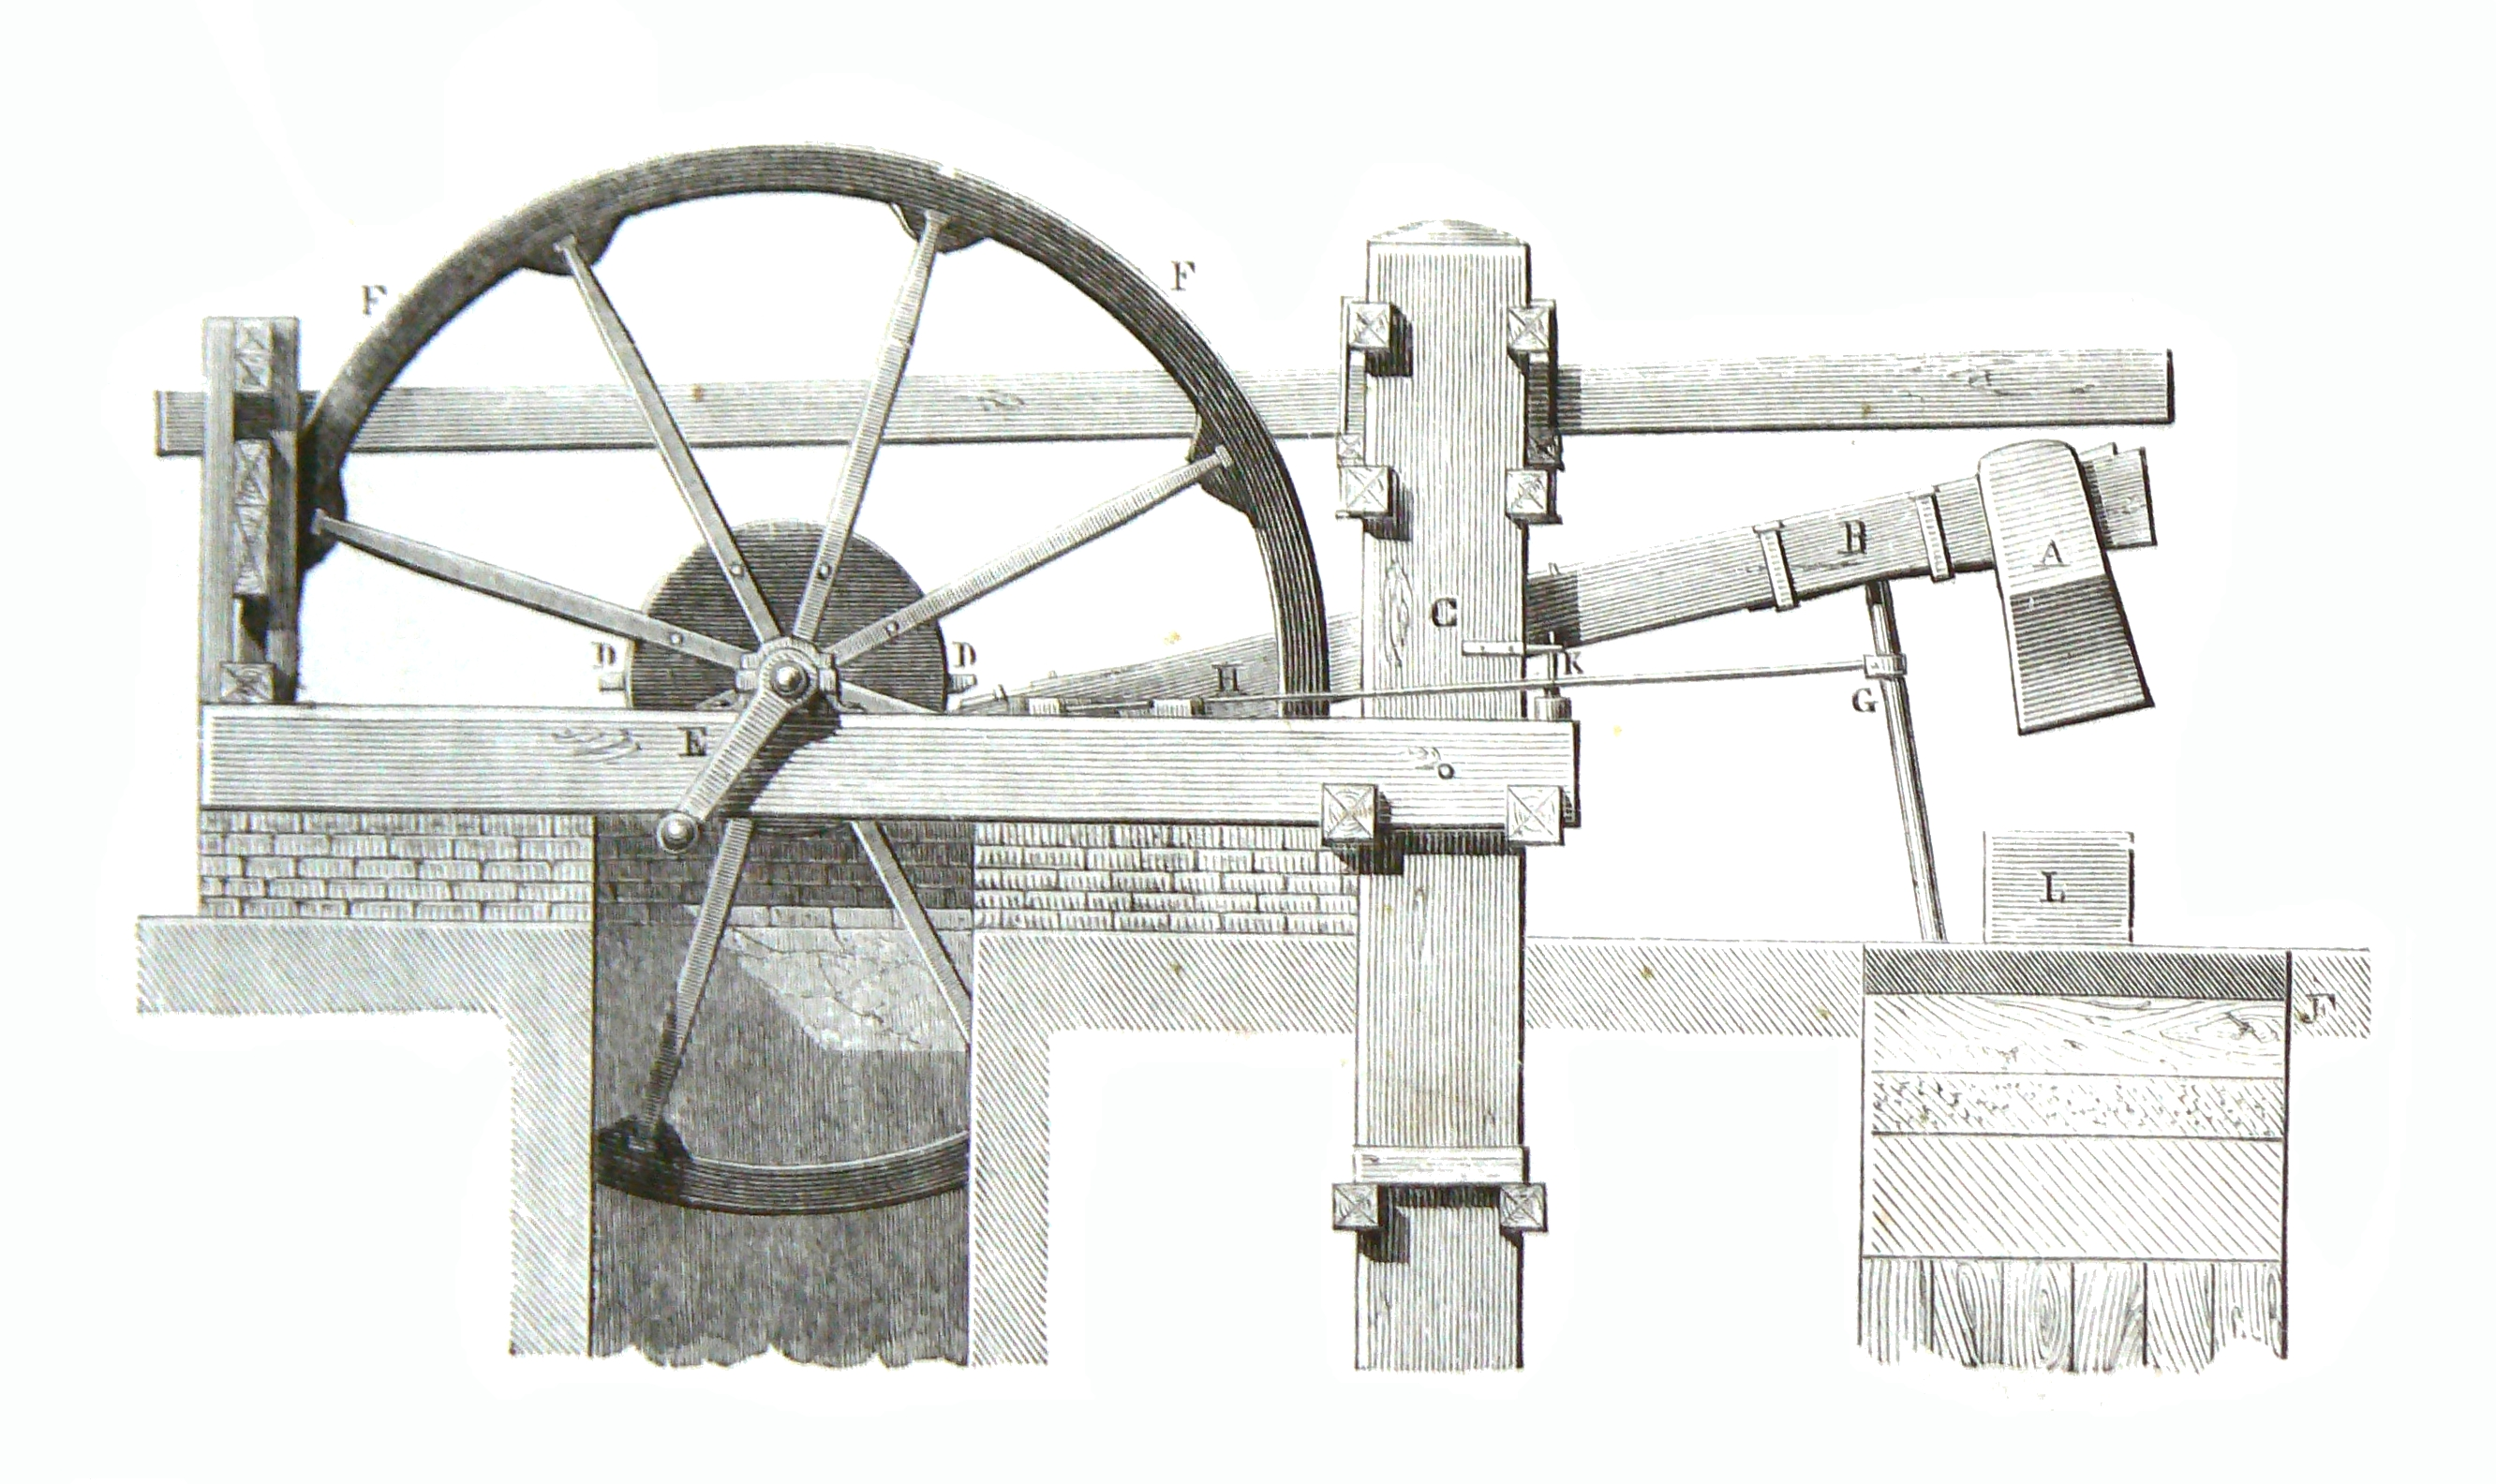
\includegraphics[width=0.8\linewidth]{blacksmith.jpg}
\end{figure}

{\small source https://commons.wikimedia.org/w/index.php?curid=1520727}

\end{center}
\end{frame}

%%%%%%%%%%%%%%%%%%%%%%%%%%%%%

\begin{frame}{Current definition: ISO 8373:2012(en)}
\begin{center}
\textbf{\large  Robots and robotic devices\\[4pt]}

Actuated mechanism (re-)programmable in two or more axes with a degree of autonomy, moving within its environment, to perform intended tasks.

\end{center}
\end{frame}

%%%%%%%%%%%%%%%%%%%%%%%%%%%%%

\begin{frame}{First manipulator - Unimate}
\begin{center}
\begin{minipage}{0.49\linewidth}
\begin{center}
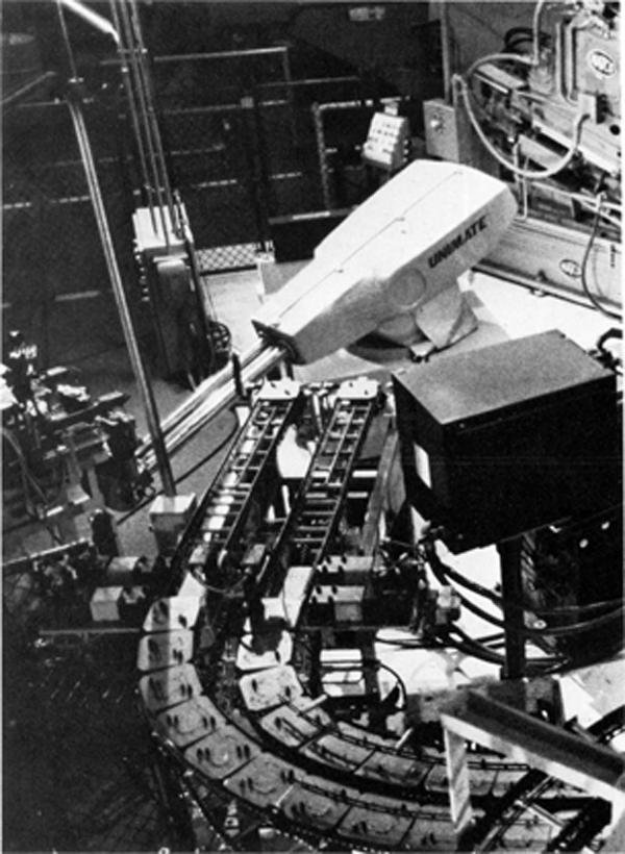
\includegraphics[width=0.8\linewidth]{unimate.png}
\end{center}
\end{minipage}
\hfill
\begin{minipage}{0.49\linewidth}
\begin{itemize}
\item Developed in the 50's
\item Industrialized in 61
\item Only predefined tasks
\end{itemize}
\end{minipage}

\end{center}
\end{frame}

%%%%%%%%%%%%%%%%%%%%%%%%%%%%%

\begin{frame}{First mobile autonomous robot - Shakey}
\begin{center}
\begin{minipage}{0.49\linewidth}
\begin{center}
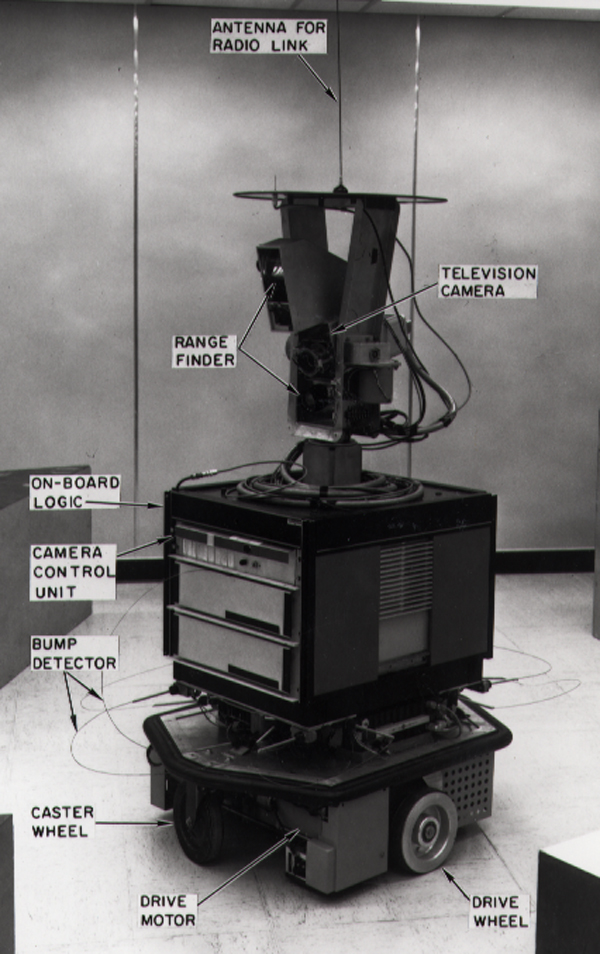
\includegraphics[width=0.8\linewidth]{SRI_Shakey_with_callouts.jpg}
\end{center}
\end{minipage}
\hfill
\begin{minipage}{0.49\linewidth}
\begin{itemize}
\item Developed from 66 to 72
\item Object recognition
\item Path and task planning
\end{itemize}
\end{minipage}

\end{center}
\end{frame}

%%%%%%%%%%%%%%%%%%%%%%%%%%%%%

\begin{frame}{First mobile autonomous robot - Shakey}
\begin{center}
\begin{minipage}{0.49\linewidth}
\begin{center}
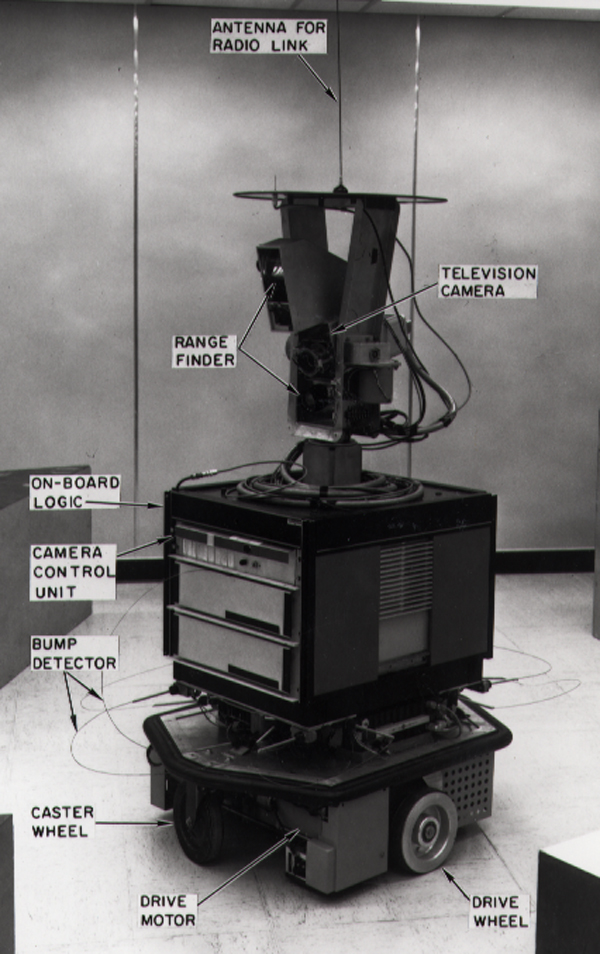
\includegraphics[width=0.8\linewidth]{SRI_Shakey_with_callouts.jpg}
\end{center}
\end{minipage}
\hfill
\begin{minipage}{0.49\linewidth}
\begin{itemize}
\item Developed from 66 to 72
\item Object recognition
\item Path and task planning
\end{itemize}
\end{minipage}

\end{center}
\end{frame}

%%%%%%%%%%%%%%%%%%%%%%%%%%%%%

\begin{frame}{Autonomous robots state of the art - Atlas}
\begin{center}
\only<1>{
	\begin{minipage}{0.49\linewidth}
	\begin{center}
	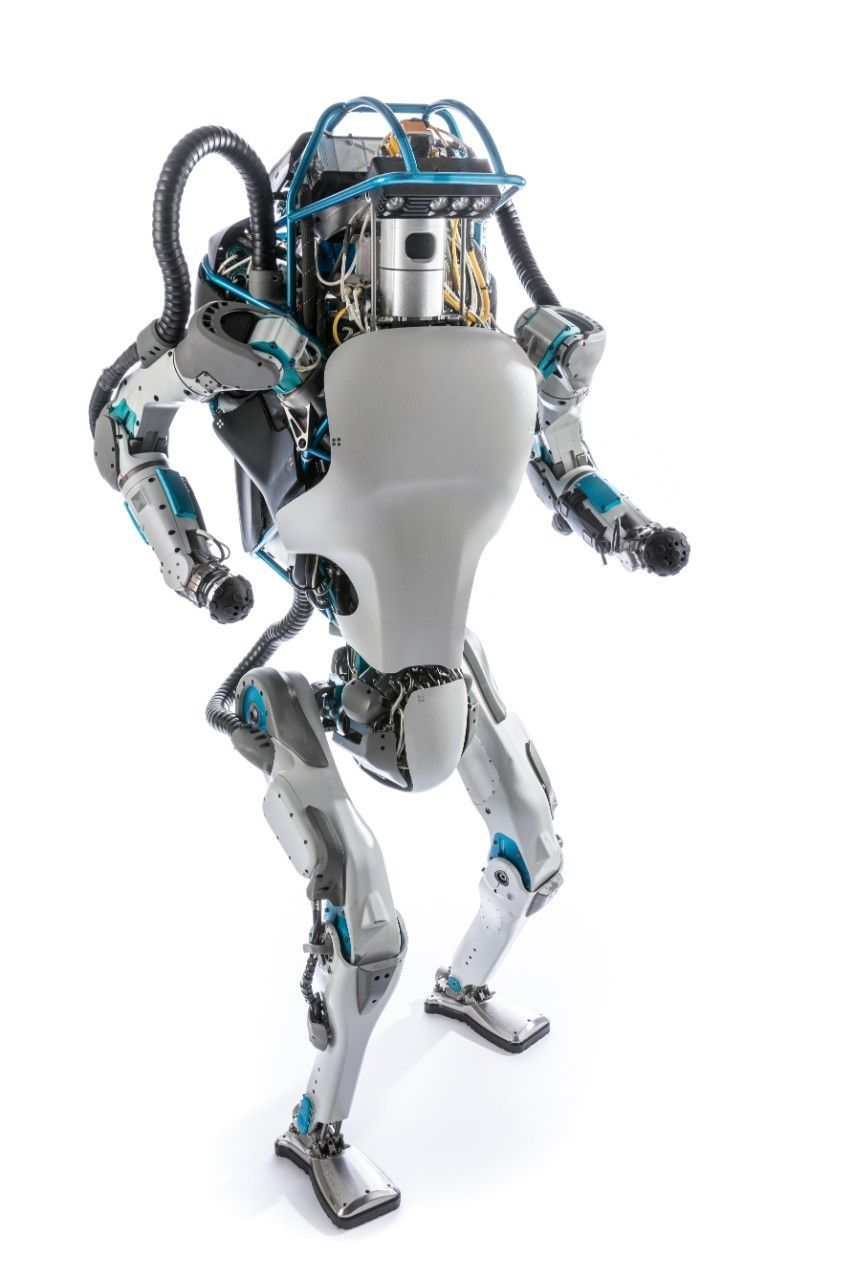
\includegraphics[width=0.8\linewidth]{Atlas_intro.jpg}
	\end{center}
	\end{minipage}
	\hfill
	\begin{minipage}{0.49\linewidth}
	\begin{itemize}
	\item Humanoid robot developed by Boston dynamics
	\item Largely autonomous
	\item Path and task planning
	\end{itemize}
	\end{minipage}
}
\only<2>{
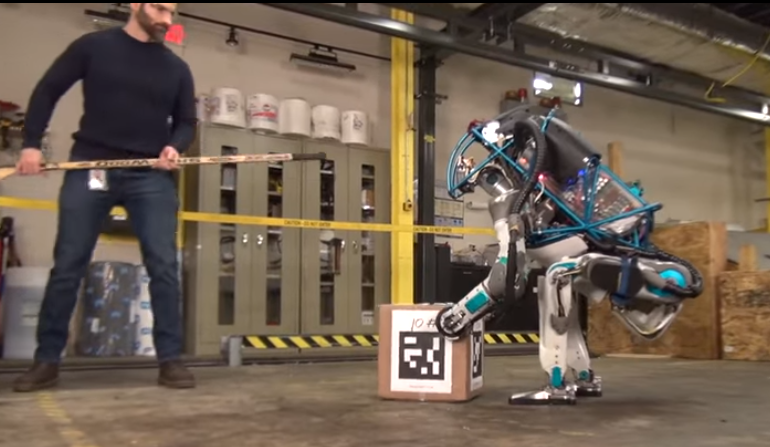
\includegraphics[width=0.99\linewidth]{Atlas_trying.png}
}
\only<3>{
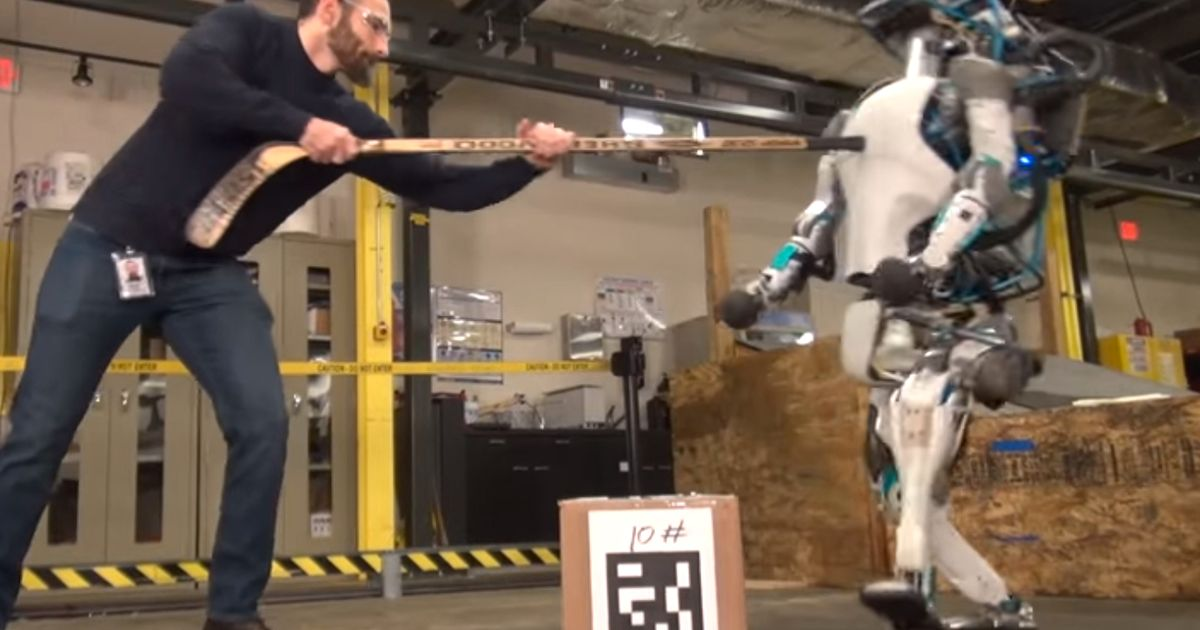
\includegraphics[width=0.99\linewidth]{Atlas_push.jpg}
}
\only<4>{
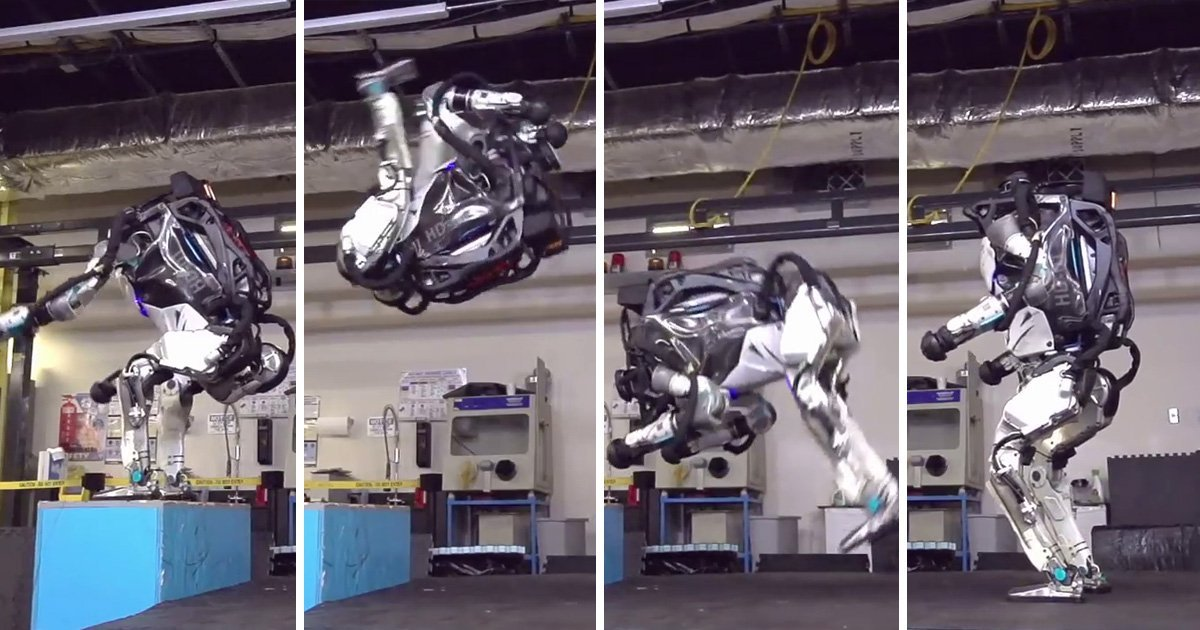
\includegraphics[width=0.99\linewidth]{Atlas_backflip.jpg}
}
\end{center}
\end{frame}

%%%%%%%%%%%%%%%%%%%%%%%%%%%%%%%%%%%%%%%%%%%%%%%%%%%%%%%%%%
\section{The control theoretic perspective}
%%%%%%%%%%%%%%%%%%%%%%%%%%%%%
\begin{frame}{Robot control - Overview}
\begin{center}
\only<1>{
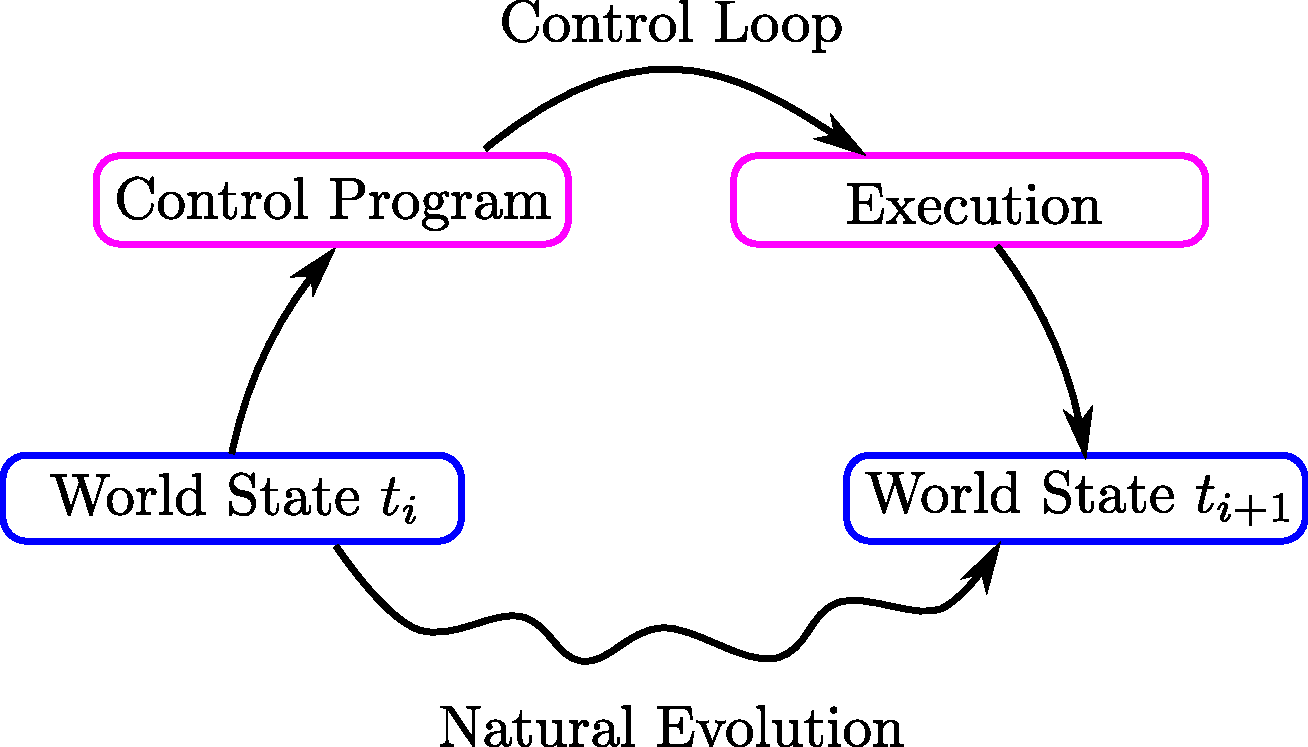
\includegraphics[width=0.7\linewidth]{control1.pdf}
}
\only<2>{
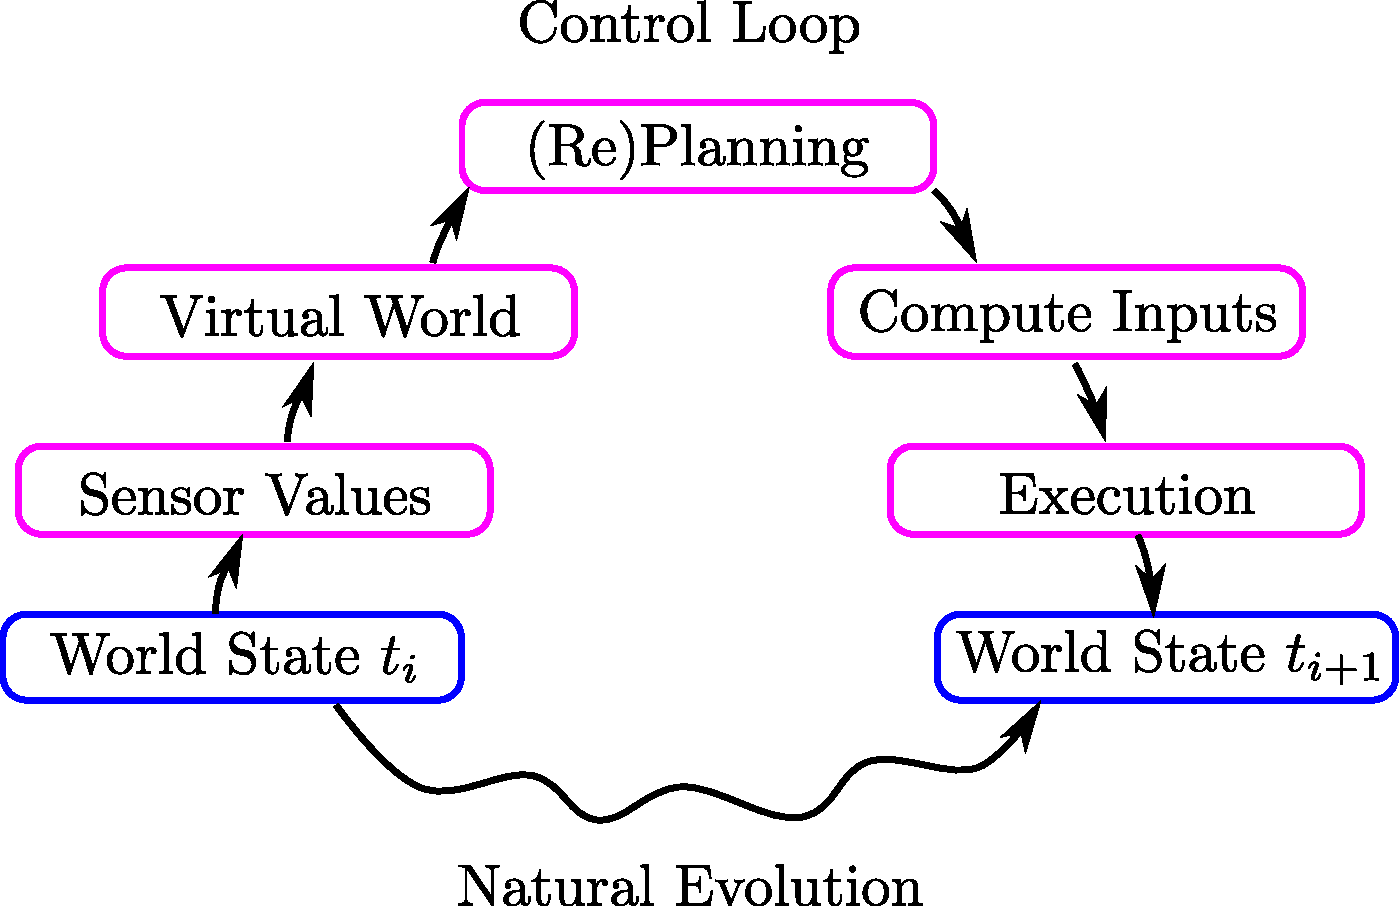
\includegraphics[width=0.85\linewidth]{control2.pdf}
}
\end{center}
\end{frame}
%%%%%%%%%%%%%%%%%%%%%%%%%%%%%
\begin{frame}{Control theory - Goal}
\begin{center}
{\large Control theory seeks means to generate control signals or inputs such that the state evolves in a desired way. }
\end{center}
\end{frame}
%%%%%%%%%%%%%%%%%%%%%%%%%%%%%
\begin{frame}{Control theory - Realization I}
\begin{center}
	\vspace{-6pt}
    \textbf{\Large Centrifugal governor\\[4pt]}
    \def\svgwidth{.5\linewidth}
    \input{regulator.pdf_tex}
    \visible<2>{
    \begin{minipage}{0.49\linewidth}
    \begin{center}
        opening angle depends on current speed
    \end{center}
    \end{minipage}
    \begin{minipage}{0.49\linewidth}
    \begin{center}
        negative feedback between opening angle and input power
    \end{center}
    \end{minipage}
    }
\end{center}
\end{frame}
%%%%%%%%%%%%%%%%%%%%%%%%%%%%%
\begin{frame}{Control theory - Concepts I}
A robot from a control theoretic perspective looks like this:
\begin{align*}
    \xd &= f(\x) + g_{\uv}(\x, \uv) + g_{{\omega_{\x}}}(\x, \omega_{\x})  \\
    \y &= h(\x, \omega_{\y})
\end{align*}
\visible<1->{
    \begin{columns}
    \begin{column}{0.5\linewidth}
        $\x$ : system state \\
        $\y$ : output state \\
        $\omega_{\x}$ : perturbations \\
        $\omega_{\y}$ : (measurement) noise
    \end{column}
    \begin{column}{0.5\linewidth}
        $f,\ g$ : system and input dynamics \\
        $\uv$ : control input \\
        $g_{{\omega_{\x}}}$ : perturbation dynamics
    \end{column}
    \end{columns}
}
\end{frame}
%%%%%%%%%%%%%%%%%%%%%%%%%%%%%
\begin{frame}{Control theory - Concepts II}
\begin{center}
\textbf{\Large Formalizing ``in a desired way''}\\[12pt]
\begin{minipage}{\linewidth}
\begin{minipage}[t]{0.49\linewidth}
	\begin{center}
	\textbf{\large Trajectory generation: }\\[4pt]
	compute a feasible trajectory
	\end{center}	
	\vfill
\end{minipage}
\hfill
\begin{minipage}[t]{0.49\linewidth}
	\begin{center}
	\textbf{\large Stabilization: }\\[4pt]
	reject perturbations and make the control ``robust''
	\end{center}
	\vfill
\end{minipage}
\visible<2>{
\begin{center}
\textbf{\large Classification of the dynamics:\\[4pt] }
\begin{minipage}[c]{\linewidth}
	\textbullet nonlinear \hfill \textbullet polynomial \hfill \textbullet linear \hfill
\end{minipage}
\end{center}
}
\end{minipage}
\end{center}
\end{frame}
%%%%%%%%%%%%%%%%%%%%%%%%%%%%%
\begin{frame}{Trajectory generation - Dubins' car}
\begin{center}
Simplified car dynamics:\\
constant forward velocity, minimal turning radius
\only<1>{
\begin{figure}
	\def\svgwidth{\linewidth}
	\input{dubins.pdf_tex}
\end{figure}
It can be shown that the ideal (shortest) trajectory between two configurations contains only straight lines and circle segments with minimal radius.
}

\only<2>{
\begin{figure}
	\def\svgwidth{.6\linewidth}
	\input{dubins_2_0.pdf_tex}
\end{figure}
By allowing for more expressive behaviour (obstacles), the problem becomes (drastically) more complicated.
}
%https://en.wikipedia.org/wiki/Dubins_path
%Johnson, H. H "An application of the maximum principle to the geometry of plane curves", Proceedings of the American Mathematical Society, 44(2):432- 435, 1974.
%Boissonat, J.D.; A. Cerezo; K. Leblond (May 1992). "Shortest Paths of Bounded Curvature in the Plane" (PDF). Proceedings of the IEEE International Conference on Robotics and Automation. 3. Piscataway, NJ. pp. 2315–2320. doi:10.1109/ROBOT.1992.220117.
\end{center}
\end{frame}
%%%%%%%%%%%%%%%%%%%%%%%%%%%%%
\begin{frame}{Trajectory generation - Randomized planning}
\only<1>{
\begin{figure}
	\def\svgwidth{\linewidth}
	\input{planning_0.pdf_tex}
\end{figure}
}
\only<2>{
\begin{figure}
	\def\svgwidth{\linewidth}
	\input{planning_1.pdf_tex}
\end{figure}
}
\only<3>{
\begin{figure}
	\def\svgwidth{.8\linewidth}
	\input{planning_2.pdf_tex}
\end{figure}
}
\only<4>{
\begin{figure}
	\def\svgwidth{.8\linewidth}
	\input{planning_3.pdf_tex}
\end{figure}
}
\only<5>{
\begin{figure}
	\def\svgwidth{.8\linewidth}
	\input{planning_4.pdf_tex}
\end{figure}
}
\end{frame}
%%%%%%%%%%%%%%%%%%%%%%%%%%%%%
\begin{frame}{Trajectory stabilization}
\begin{center}
Trajectory generators give us a reference trajectory and in an ideal world we could simply replay the inputs $\uv(t)$.\\
\visible<2->{This is called open-loop control\\[4pt]}
\visible<3->{Sadly the world isn't perfect: modelling errors, noise, friction, ...}
\visible<4->{
\begin{figure}
	\def\svgwidth{.8\linewidth}
	\input{trajectory_stab_1.pdf_tex}	
\end{figure}
Compute a control law $g(\delta\x)$ s.t. the system trajectory converges to its reference
}
\end{center}
\end{frame}
%%%%%%%%%%%%%%%%%%%%%%%%%%%%%
\begin{frame}{Trajectory stabilization - optimal control}
% https://stanford.edu/class/ee363/lectures/dlqr.pdf
% https://ocw.mit.edu/courses/mechanical-engineering/2-154-maneuvering-and-control-of-surface-and-underwater-vehicles-13-49-fall-2004/lecture-notes/lec19.pdf
\begin{center}
Consider the discrete-time linear system:
\begin{equation*}
\x_i = A.\x_{i-1} + B.\uv_{i-1}
\end{equation*}
and optimality defined by the cost function
\begin{equation}
J(\x_0) = \sum_{{i=0}}^{{N-1}}\left(\xT_i.Q.\x_i + \tp{\uv}_i.R.\uv_i\right) + \xT_N.Q.\x_N
\end{equation}
Possible methods to obtain the Linear Quadratic Regulator (LQR):\\[6pt]
\begin{minipage}[c]{0.5\linewidth}
\begin{itemize}
\item via Least-Squares
\item via Dynamic Programming
\item via Convex Optimization
\end{itemize}
\end{minipage}
\end{center}
\end{frame}

%%%%%%%%%%%%%%%%%%%%%%%%%%%%%
\begin{frame}{Optimal control - Dynamic Programming}
\begin{center}
A solution can be found using dynamic programming and iterating from end to start.\\[4pt]

The final cost is ``fixed'': $J(\x_N) = \xT_N.Q.\x_N$ \\[4pt]
\visible<2->{
	The cost for $i=N-1$ is:\\[4pt]
	$J(\x_{N-1}) = \xT_{N-1}.Q.\x_{N-1} + \tp{\uv}_{N-1}.R.\uv_{N-1} + \xT_N.Q.\x_N$\\
	and moreover $\x_i = A.\x_{i-1} + B.\uv_{i-1}$
} 
\visible<3->{ so we get:\\[4pt]
$J(\x_{N-1}) = \xT_{N-1}.Q.\x_{N-1} + \tp{\uv}_{N-1}.R.\uv_{N-1} + J(A.\x_{i-1} + B.\uv_{i-1})$\\
}

\end{center}
\end{frame}

%%%%%%%%%%%%%%%%%%%%%%%%%%%%%
\begin{frame}{Optimal control - Dynamic Programming}
\begin{center}

This means that we can solve the problem by recursively solving :\\[4pt]
$\uv_{N-1} = \argmin_\uv \tp{\uv}.R.\uv + J(A.\x_{i-1} + B.\uv)$

\end{center}
\end{frame}


%%%%%%%%%%%%%%%%%%%%%%%%%%%%%%%%%%%%%%%%%%%%%%%%%%%%%%%%%%


\section{The industrial perspective}
\begin{frame}{The industrial perspective}
\begin{center}
    \Large{\textcolor{blue}{Three main applications}}
    \def\svgwidth{\linewidth}
    \input{industrial_robots1.pdf_tex}
\end{center}
\end{frame}

%%%%%%%%%%%%%%%%%%%%%%%%%%%%%
\begin{frame}{Robotic arm}
    \begin{center}
        \begin{minipage}{0.49\linewidth}
                \def\svgwidth{\linewidth}
                \input{robotic_arms.pdf_tex}
        \end{minipage}
        \hfill
        \begin{minipage}{0.49\linewidth}
        \large{Serial link robotic arm}
        \begin{itemize}
            \pro Large work-space
            \pro Versatility
            \item[]
            \con Complexity due to redundancy
            \con Relatively slow
        \end{itemize}
        \end{minipage}
    \end{center}
\end{frame}

\begin{frame}{Robotic arm - Frequent use case}
    \begin{center}
     % Video here
    \end{center}
\end{frame}
%%%%%%%%%%%%%%%%%%%%%%%%%%%%%
\begin{frame}{Parallel robot}
    \begin{center}
        \begin{minipage}{0.49\linewidth}
                \def\svgwidth{\linewidth}
                \input{pick_and_place.pdf_tex}
        \end{minipage}
        \hfill
        \begin{minipage}{0.49\linewidth}
        \large{Serial link robotic arm}
        \begin{itemize}
            \pro Speed \& precision
            \pro Large 	work-space
            \item[]
            \con Complexity due to internal constraints
            \con Restricted orientation
        \end{itemize}
        \end{minipage}
    \end{center}
\end{frame}

\begin{frame}{Parallel robot - Frequent use case}
    \begin{center}
     % Video here
    \end{center}
\end{frame}
%%%%%%%%%%%%%%%%%%%%%%%%%%%%%
\begin{frame}{Mobile robots}
    \begin{center}
        \begin{minipage}{0.49\linewidth}
                \def\svgwidth{\linewidth}
                \input{logistics_1.pdf_tex}
        \end{minipage}
        \hfill
        \begin{minipage}{0.49\linewidth}
        \large{Serial link robotic arm}
        \begin{itemize}
            \pro Increases efficiency in warehouses
            \pro Semi-autonomous systems
            \item[]
            \con Complexity due to multi-agent nature
            \con Very task specific
        \end{itemize}
        \end{minipage}
    \end{center}
\end{frame}

\begin{frame}{Mobile robot - Use case}
    \begin{center}
     % Video here
    \end{center}
\end{frame}
%%%%%%%%%%%%%%%%%%%%%%%%%%%%%

\begin{frame}[plain]

\begin{center}
\textbf{\Large Robotics from various perspectives}\\[6pt]
Philipp Schlehuber-Caissier
\end{center}
	
\end{frame}

%%%%%%%%%%%%%%%%%%%%%%%%%%%%%%%%%%%%%%%%%%%%%%%%%%%%%%%%

\end{document}

